\documentclass{article}\usepackage[]{graphicx}\usepackage[]{color}
%% maxwidth is the original width if it is less than linewidth
%% otherwise use linewidth (to make sure the graphics do not exceed the margin)
\makeatletter
\def\maxwidth{ %
  \ifdim\Gin@nat@width>\linewidth
    \linewidth
  \else
    \Gin@nat@width
  \fi
}
\makeatother

\definecolor{fgcolor}{rgb}{0.345, 0.345, 0.345}
\newcommand{\hlnum}[1]{\textcolor[rgb]{0.686,0.059,0.569}{#1}}%
\newcommand{\hlstr}[1]{\textcolor[rgb]{0.192,0.494,0.8}{#1}}%
\newcommand{\hlcom}[1]{\textcolor[rgb]{0.678,0.584,0.686}{\textit{#1}}}%
\newcommand{\hlopt}[1]{\textcolor[rgb]{0,0,0}{#1}}%
\newcommand{\hlstd}[1]{\textcolor[rgb]{0.345,0.345,0.345}{#1}}%
\newcommand{\hlkwa}[1]{\textcolor[rgb]{0.161,0.373,0.58}{\textbf{#1}}}%
\newcommand{\hlkwb}[1]{\textcolor[rgb]{0.69,0.353,0.396}{#1}}%
\newcommand{\hlkwc}[1]{\textcolor[rgb]{0.333,0.667,0.333}{#1}}%
\newcommand{\hlkwd}[1]{\textcolor[rgb]{0.737,0.353,0.396}{\textbf{#1}}}%
\let\hlipl\hlkwb

\usepackage{framed}
\makeatletter
\newenvironment{kframe}{%
 \def\at@end@of@kframe{}%
 \ifinner\ifhmode%
  \def\at@end@of@kframe{\end{minipage}}%
  \begin{minipage}{\columnwidth}%
 \fi\fi%
 \def\FrameCommand##1{\hskip\@totalleftmargin \hskip-\fboxsep
 \colorbox{shadecolor}{##1}\hskip-\fboxsep
     % There is no \\@totalrightmargin, so:
     \hskip-\linewidth \hskip-\@totalleftmargin \hskip\columnwidth}%
 \MakeFramed {\advance\hsize-\width
   \@totalleftmargin\z@ \linewidth\hsize
   \@setminipage}}%
 {\par\unskip\endMakeFramed%
 \at@end@of@kframe}
\makeatother

\definecolor{shadecolor}{rgb}{.97, .97, .97}
\definecolor{messagecolor}{rgb}{0, 0, 0}
\definecolor{warningcolor}{rgb}{1, 0, 1}
\definecolor{errorcolor}{rgb}{1, 0, 0}
\newenvironment{knitrout}{}{} % an empty environment to be redefined in TeX

\usepackage{alltt}
\usepackage{enumitem}
\usepackage{ amssymb }
\usepackage{ textcomp }
\usepackage{longtable}
\usepackage{amsmath,tabu}
\usepackage{caption}
\usepackage{subcaption}
\usepackage{float}
\usepackage[figurename=Supplemental Figure]{caption}
\usepackage{titling}

\setlength{\droptitle}{-5em}  
\topmargin=-0.4in
\evensidemargin=0in
\oddsidemargin=0in
\textwidth=6.5in
\textheight=9in
\headsep=0.25in

\title{Interrogation of human hematopoietic traits at single-cell and single-variant resolution}
\date{Supplemental Information}
\author{(Caleb, Erik, Jacob), Will?, Hilary, Joel, (Martin, Jason, Vijay)}
\IfFileExists{upquote.sty}{\usepackage{upquote}}{}
\begin{document}
\maketitle
\section*{Overview of UK Biobank data}
\begin{enumerate}[label=(\Alph*)]
\item 
a
\begin{knitrout}
\definecolor{shadecolor}{rgb}{0.969, 0.969, 0.969}\color{fgcolor}\begin{figure}[H]

{\centering 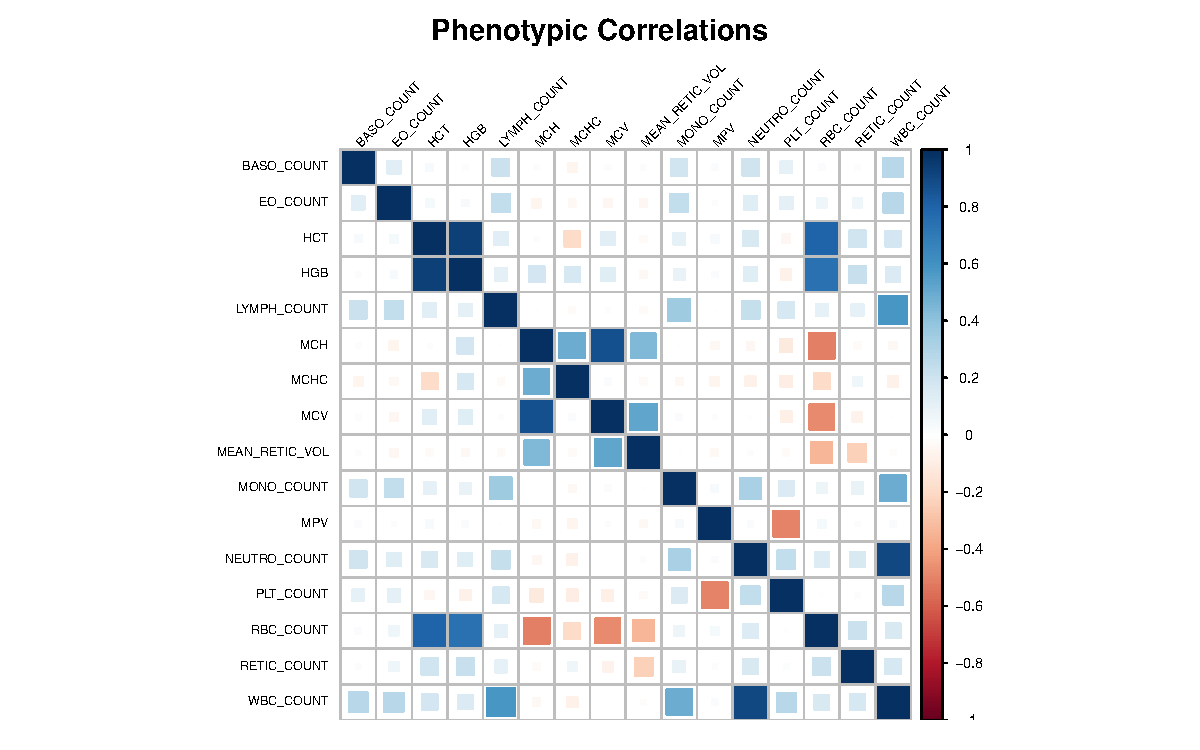
\includegraphics[width=\maxwidth]{figure/correlationPlots-1} 

}

\caption[Fold change enrichment of individually resolved peaks]{Fold change enrichment of individually resolved peaks}\label{fig:correlationPlots1}
\end{figure}

\begin{kframe}

{\ttfamily\noindent\bfseries\color{errorcolor}{\#\# Error in file(file, "{}rt"{}): cannot open the connection}}

{\ttfamily\noindent\bfseries\color{errorcolor}{\#\# Error in gc.matrix[i, j]: incorrect number of dimensions}}

{\ttfamily\noindent\bfseries\color{errorcolor}{\#\# Error in gc.matrix[i, j]: incorrect number of dimensions}}

{\ttfamily\noindent\bfseries\color{errorcolor}{\#\# Error in corrplot(output, method = "{}square"{}, order = "{}hclust"{}, hclust.method = "{}complete"{}, : object 'output' not found}}\end{kframe}\begin{figure}[H]

{\centering 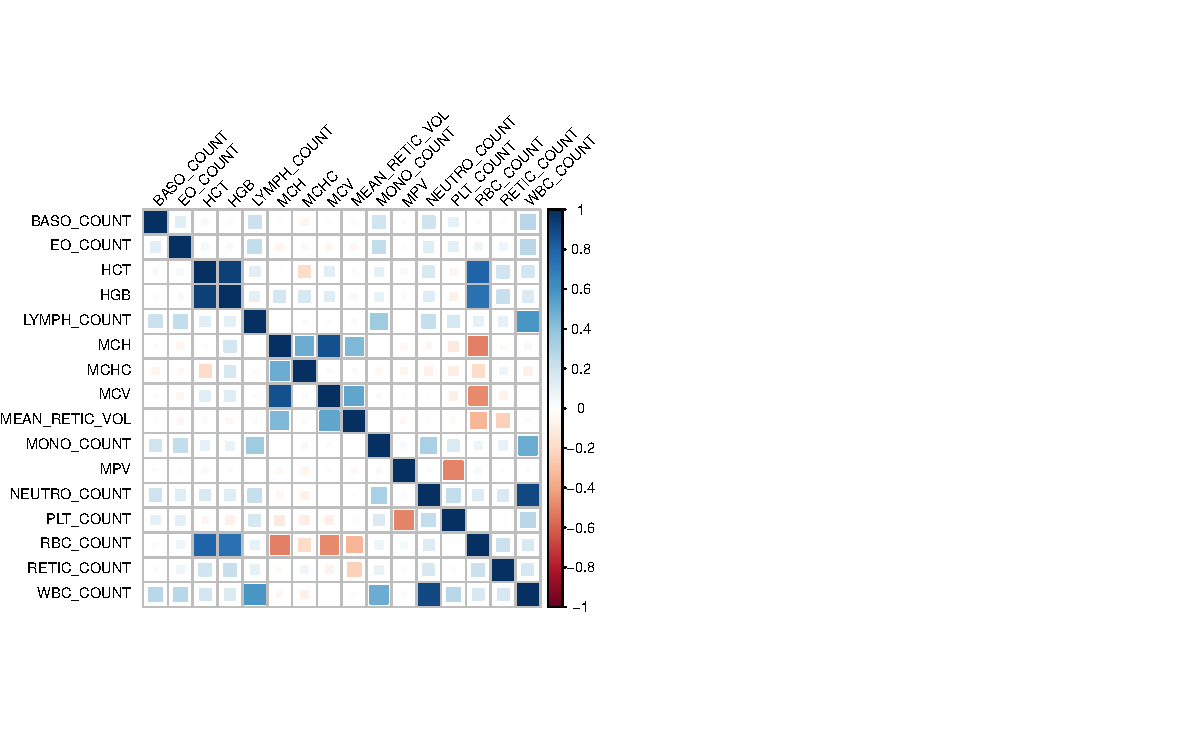
\includegraphics[width=\maxwidth]{figure/correlationPlots-2} 

}

\caption[Fold change enrichment of individually resolved peaks]{Fold change enrichment of individually resolved peaks}\label{fig:correlationPlots2}
\end{figure}

\begin{kframe}

{\ttfamily\noindent\bfseries\color{errorcolor}{\#\# Error in corrplot(output, method = "{}square"{}, order = "{}hclust"{}, tl.cex = 0.6, : object 'output' not found}}

{\ttfamily\noindent\bfseries\color{errorcolor}{\#\# Error in eval(expr, envir, enclos): object 'output' not found}}

{\ttfamily\noindent\bfseries\color{errorcolor}{\#\# Error in genotriangle[lower.tri(genotriangle, diag = FALSE)] <- 0: object 'genotriangle' not found}}

{\ttfamily\noindent\bfseries\color{errorcolor}{\#\# Error in melt(phenotriangle): could not find function "{}melt"{}}}

{\ttfamily\noindent\bfseries\color{errorcolor}{\#\# Error in melt(genotriangle): could not find function "{}melt"{}}}

{\ttfamily\noindent\bfseries\color{errorcolor}{\#\# Error in melt(phenocors): could not find function "{}melt"{}}}

{\ttfamily\noindent\bfseries\color{errorcolor}{\#\# Error in paste(genomelt\$Var1, genomelt\$Var2): object 'genomelt' not found}}

{\ttfamily\noindent\bfseries\color{errorcolor}{\#\# Error in paste(phenomelt\$Var1, phenomelt\$Var2): object 'phenomelt' not found}}

{\ttfamily\noindent\bfseries\color{errorcolor}{\#\# Error in colnames(genomelt)[3] <- "{}GenoCor"{}: object 'genomelt' not found}}

{\ttfamily\noindent\bfseries\color{errorcolor}{\#\# Error in colnames(phenomelt)[3] <- "{}PhenoCor"{}: object 'phenomelt' not found}}

{\ttfamily\noindent\bfseries\color{errorcolor}{\#\# Error in merge(genomelt, phenomelt, by = "{}traitpairs"{}): object 'genomelt' not found}}

{\ttfamily\noindent\bfseries\color{errorcolor}{\#\# Error in merged[, c("{}Var1.x"{}, "{}Var2.x"{})] <- NULL: object 'merged' not found}}

{\ttfamily\noindent\bfseries\color{errorcolor}{\#\# Error in eval(expr, envir, enclos): object 'merged' not found}}

{\ttfamily\noindent\bfseries\color{errorcolor}{\#\# Error in is.data.frame(data): object 'merged' not found}}

{\ttfamily\noindent\bfseries\color{errorcolor}{\#\# Error in attach(merged): object 'merged' not found}}

{\ttfamily\noindent\bfseries\color{errorcolor}{\#\# Error in ggplot(merged, aes(x = GenoCor, y = PhenoCor, pairs = traitpairs)): object 'merged' not found}}

{\ttfamily\noindent\bfseries\color{errorcolor}{\#\# Error: Column `h2\_obs` not found}}

{\ttfamily\noindent\bfseries\color{errorcolor}{\#\# Error in FUN(X[[i]], ...): object 'h\_obs' not found}}\end{kframe}\begin{figure}[H]

{\centering 
\includegraphics[width=\maxwidth]{figure/correlationPlots-3} 

}

\caption[Fold change enrichment of individually resolved peaks]{Fold change enrichment of individually resolved peaks}\label{fig:correlationPlots3}
\end{figure}


\end{knitrout}
\item

\begin{figure}[H]
\centering
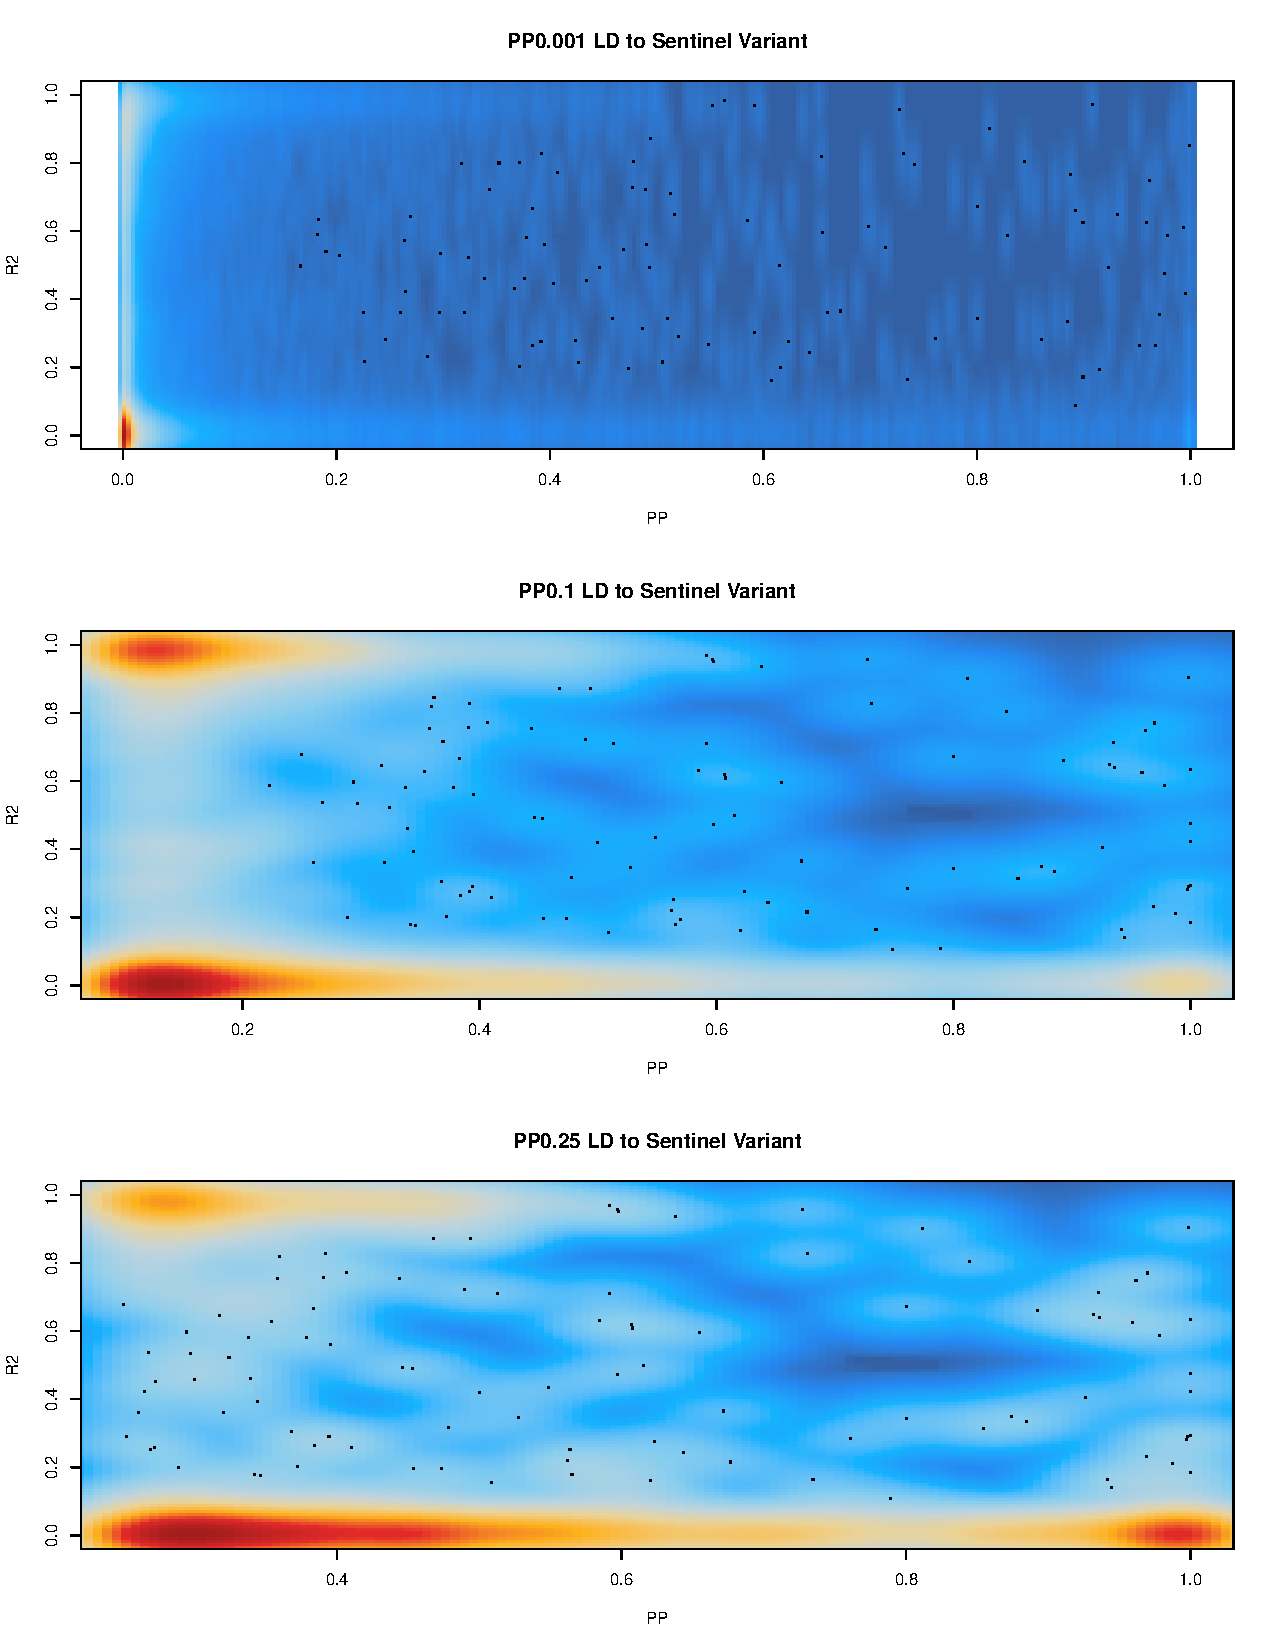
\includegraphics[width=\linewidth]{staticFigures/LDtoSentinel_PPcomparison.pdf}
\caption{Sample embedding of figure in document.}
\end{figure} 

\end{enumerate}



\section*{Description of single-cell enrichment}

\begin{knitrout}
\definecolor{shadecolor}{rgb}{0.969, 0.969, 0.969}\color{fgcolor}\begin{kframe}
\begin{alltt}
\hlkwd{print}\hlstd{(}\hlstr{"part2"}\hlstd{)}
\end{alltt}
\begin{verbatim}
## [1] "part2"
\end{verbatim}
\end{kframe}
\end{knitrout}

\end{document}
